%% If you have any problems using this template, please contact the author: %%
%% timhosgood@gmail.com %%

%% Original source: https://www.maths.ox.ac.uk/members/it/faqs/latex/presentations
%% Modified by Paulo Chiliguano
%% github.com/pauloesteban

\documentclass[xcolor=table]{beamer}
\usepackage[utf8]{inputenc}
\usepackage{charter}
\usepackage{tikz}
\usepackage{graphicx}
\usepackage{amsmath}
\usepackage{amssymb}
\usepackage{tcolorbox}

\usepackage[labelformat=empty,font=scriptsize,skip=0pt,justification=justified,singlelinecheck=false]{caption}

%% remove the icon
\setbeamertemplate{bibliography item}{}

%% remove line breaks
\setbeamertemplate{bibliography entry title}{}
\setbeamertemplate{bibliography entry location}{}
\setbeamertemplate{bibliography entry note}{}

%% change the caption name
\renewcommand{\figurename}{Figura}

%% Title slide formatting %%

\pgfdeclareimage[width=\paperwidth]{titlebackground}{images/6780418194_7873366e90_o.jpg}
\setbeamerfont{subtitle}{size=\tiny}
\setbeamertemplate{title page}{
    \begin{picture}(0,0)
        \put(-28.5,-163){%
            \pgfuseimage{titlebackground}
        }
        \put(0,-75){%
            \begin{minipage}[b][4.5cm][t]{0.70\textwidth}
                \color{udlacolour}
                \usebeamerfont{title}
                    {\inserttitle\\[0.9cm]}
                \usebeamerfont{subtitle}
                    {\insertauthor\par}
                    {\insertinstitute\\[0.3cm]}
                    {\insertdate}
            \end{minipage}
        }
    \end{picture}
}



%% General slide formatting %%

\definecolor{udlacolour}{RGB}{127,5,19}

%\pgfdeclareimage[width=0.8cm]{uteqlogo}{images/logoUTEQdegradado.png}
%\pgfdeclareimage[width=0.8cm]{fcamblogo}{images/logo_fcamb.jpg}

\setbeamertemplate{headline}
{%
    \begin{picture}(0,0)
        %\put(314,-40){%
            %\pgfuseimage{uteqlogo}
        %}
        \put(20,-45){%
            \rule{320pt}{0.4pt}
        }
    \end{picture}
}

\setbeamertemplate{frametitle}
{%
    \begin{picture}(0,0)
        \put(-8,-10){%
            \normalsize\color{udlacolour}\insertframetitle
        }
        \put(-7,-20){%
            \tiny\color{udlacolour}\insertframesubtitle
        }
    \end{picture}
}

\setbeamertemplate{footline}
{%
    \begin{picture}(0,0)
        \put(20,30){%
            \rule{320pt}{0.4pt}
        }
        %\put(20,14){%
            %\pgfuseimage{fcamblogo}
        %}
        \put(100,14){%
            \color{udlacolour}\insertshortdate
        }
        \put(160,14){%
            \color{udlacolour}\insertshorttitle
        }
        \put(337,14){%
            \color{udlacolour}\insertpagenumber
        }
    \end{picture}%
}



%% Information (author, title, etc.) %%

\title[Planeación y desarrollo de carrera en Music Business]{Planeación y desarrollo de carrera en Music Business} % short title for footer
\author%
{%
    \sc{Paulo Chiliguano}\\
    \textit{MSc in Sound and Music Computing}
}
\institute%
{%
    \textit{Queen Mary University of London}
}
\date[Octubre 2018]{16 de octubre de 2018} % short date for footer



%% Content of slides %%

\begin{document}
	\begin{frame}[plain]
		\titlepage
	\end{frame}
	%
	\begin{frame}
		\frametitle{Contenido}
    		\tableofcontents
	\end{frame}
	%
	\section{Introducción}
	\begin{frame}
		\frametitle{Introducción}
		La industria musical está en continua evolución pero los fundamentos del negocio son constantes:
		\framesubtitle{La música y la sociedad}
		\begin{itemize}
			\item Creación
			\item Publicación
			\item Márketing
			\item Distribución
			\item Ventas
		\end{itemize}
		La tecnología digital ha hecho de la música un negocio para emprendedores debido al acceso a producción asequible y distribución con menos requerimientos de manufactura y distribución física.
	\end{frame}
	%
	\begin{frame}
		\frametitle{Music Business}
		\framesubtitle{Sistema y principales subsistemas~\cite{baskerville2006music}}
		\begin{figure}
    			\centering
    			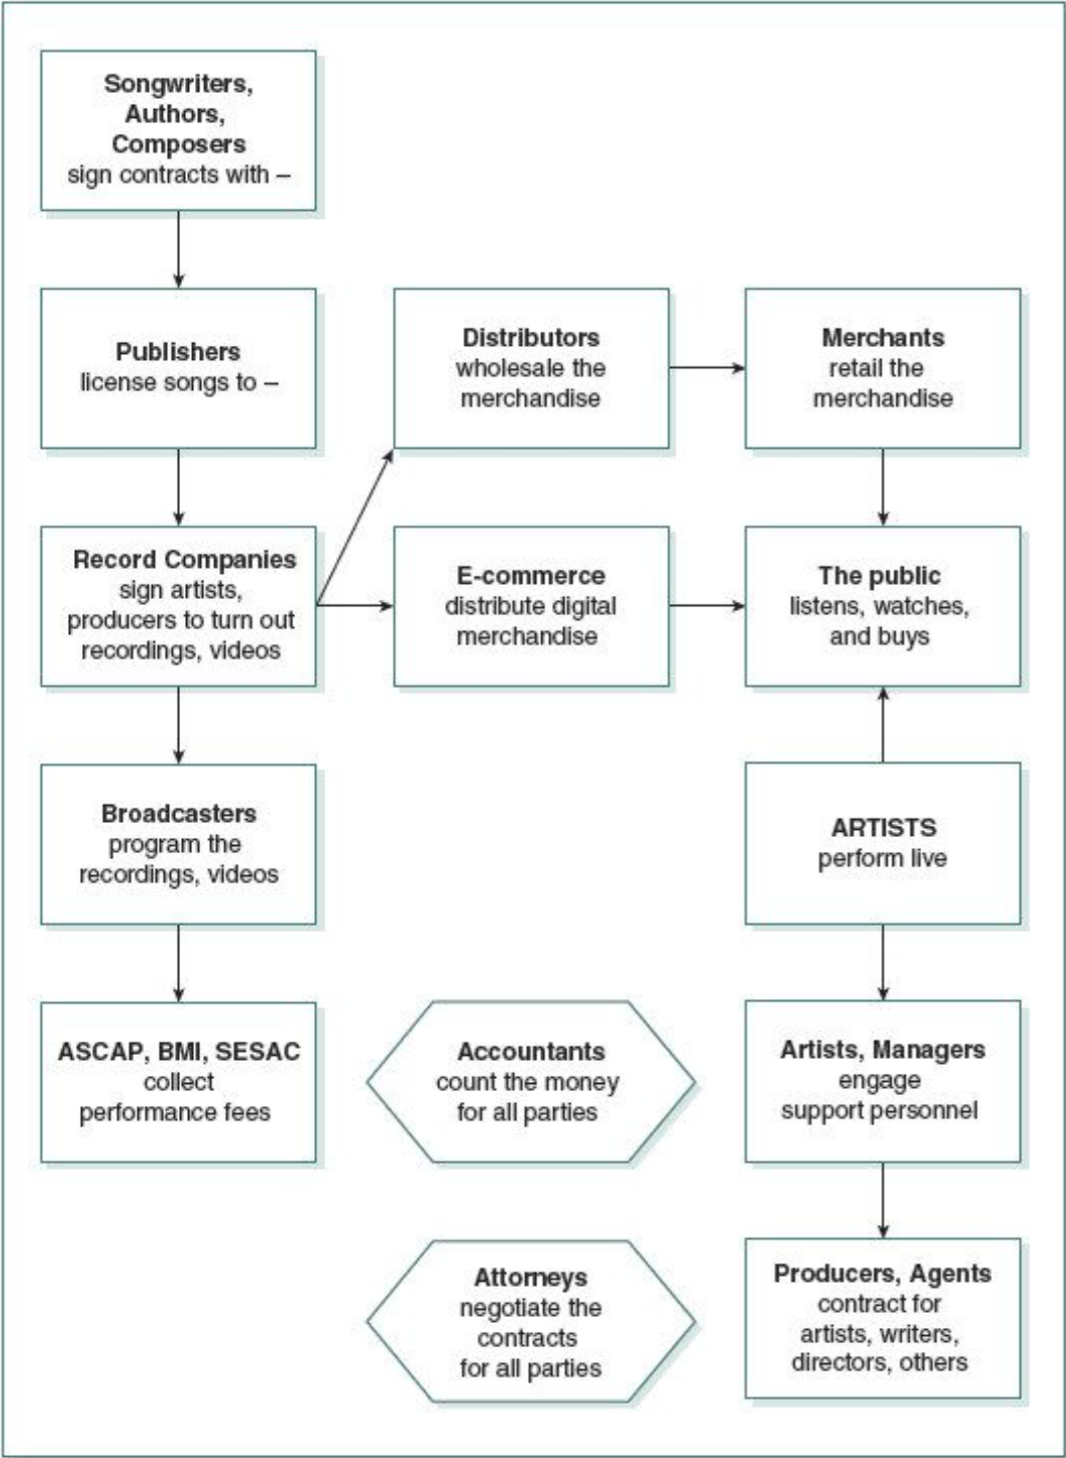
\includegraphics[scale=0.25]{images/musicbusiness.png}
    			%\caption{Sistema de \textit{music business}~\cite{baskerville2006music}}
			\label{fig:1}
    		\end{figure}
	\end{frame}
	%
	\section{Productos musicales}
	\begin{frame}
		\frametitle{Productos musicales}
		\framesubtitle{Bienes y música impresa}
		\begin{itemize}
			\item Instrumentos de teclado acústicos y electrónicos
			\item Instrumentos de viento, bronce, percusión y cuerda
			\item Equipamiento de grabación y amplificación
			\item Productos basados en computador y productos electrónicos
			\item Video juegos~\cite{passman2011all} (Guitar Hero, Rock Band)
		\end{itemize}
	\end{frame}
	%
	\begin{frame}
		\frametitle{Teclados}
		\framesubtitle{Ofrecen una amplia variedad de combinación de sonidos}
		\begin{tcolorbox}[colback=white,colframe=udlacolour,title=MIDI]
    			Interfaz digital de instrumentos musicales
    		\end{tcolorbox}
		La estandarización de MIDI permite la comunicación entre diferentes instrumentos electrónicos de manera fácil y con un menor costo.
	\end{frame}
	%
	\subsection{Promoción de productos musicales}
	\begin{frame}
		\frametitle{Promoción de productos musicales}
		\framesubtitle{La inversión se respalda en los recursos de manufactura}
		\begin{itemize}
			\item Ad cooperativo: el costo de la publicidad es compartido entre el manufacturador y vendedor.
			\item Epocas de rebajas (Black Friday).
			\item Convenciones, encuentros profesionales y clínicas musicales.
		\end{itemize}
		\begin{figure}[h]
    			%\centering
    			
\includegraphics[scale=0.50]{images/namm.png}
    			\label{fig:2}
    		\end{figure}
		\begin{columns}[t]
			\column{.5\textwidth}
			\centering
    			
\includegraphics[scale=0.10]{images/audio-developer-conference-2017_cover2.jpg}
    			\label{fig:3}
			\column{.5\textwidth}
			\centering
    			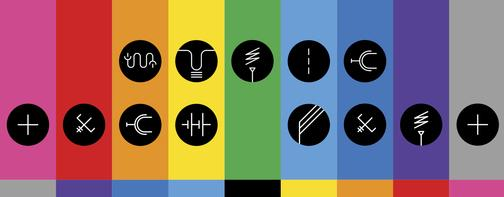
\includegraphics[scale=0.50]{images/Music_Tech_Fest.jpg}
    			\label{fig:4}
    		\end{columns}
	\end{frame}
	%
	\section{Librerías de producción musical}
	\begin{frame}
		\frametitle{Librerías de producción musical}
		\framesubtitle{Efectos de sonido y música originales}
		\begin{tcolorbox}[colback=white,colframe=udlacolour,title=Cue]
    			Cada uso que se le da requiere licenciamiento para un proyecto en específico.
    		\end{tcolorbox}
		Algunas librerías "gratuitas" hacen dinero mediante regalías (TV, radio) y licencias mecánicas. 
	\end{frame}
	%
	\section{Opciones de carrera}
	\begin{frame}
    		\frametitle{Opciones de carrera}
    		\framesubtitle{Considerar los múltiples puntos en que se interseca la música con la industria del entretenimiento}
		\begin{itemize}
			\item Creativos
			\item Directores y productores
			\item Intérpretes
			\item Educadores
			\item Radio, TV, Cine, Video juegos
		\end{itemize}
	\end{frame}
	%
	\subsection{Carreras relacionadas}
	\begin{frame}[allowframebreaks]
    		\frametitle{Carreras relacionadas}
		\framesubtitle{Mayores oportunidades para quienes aman la música y la tecnología}
		\begin{tcolorbox}[colback=white,colframe=udlacolour,title=Ingenierio de audio]
    			Profesionales con bases de ingeniería eléctrica, física, audiología, acústica y ciencias de la computación.
    		\end{tcolorbox}
		
		Se involucran en la investigación y desarrollo de equipos de audio, diseño de estudios, mastering, mantenimiento, y mezcla de sonido.
		\begin{tcolorbox}[colback=white,colframe=udlacolour,title=Inventores/Reparadores de instrumentos]
    			Personas interesadas en la Física del sonido, acústica, y electrónica.
    		\end{tcolorbox} 
		Existe escasez de personal de mantenimiento de teclados electrónicos. Tener formación musical es una ventaja.
		
		\begin{tcolorbox}[colback=white,colframe=udlacolour,title=Desarrolladores de música en línea]
    			Individuos talentosos para subir y mantener sitios web, codificar música, manejo de contenido y experiencia de usuario, y soporte técnico.
    		\end{tcolorbox}
		Conocimiento en música y estadística permiten posicionarse como analista en compañías de cualquier tamaño.
	\end{frame}
	%
	\subsection{Emprendimiento}
	\begin{frame}
		\frametitle{Emprendimiento}
		\framesubtitle{Acompañado de destrezas en contabilidad, márketing, operaciones y el arte de vender}
		\begin{itemize}
			\item ¿Cuál es el producto/servicio planeado?~\cite{ries2018lean}
			\item ¿Quién dirigirá la compañía?
			\item ¿Qué recursos se necesitan?
			\item ¿Quiénes son los consumidores y cómo se va a llegar a ellos?
			\item ¿Cuál es el tamaño del mercado objetivo y qué tan rápido está creciendo?
			\item ¿Cómo se distribuirá el negocio o servicio?
			\item ¿Cuál es el panorama competitivo y regulatorio?
			\item ¿Cuándo la compañía producirá retorno de inversión?
			\item ¿Cómo se ven afectados los inversores si se aumenta el capital?
			\item ¿Cuál es el plan de contingencia si el negocio va mal?
		\end{itemize}
	\end{frame}
	%
	\section{Desarrollo de carrera}
	\begin{frame}
    		\frametitle{Desarrollo de carrera}
		\framesubtitle{Es importante distinguir entre un trabajo y una carrera}
		\begin{table}[]
			\begin{tabular}{|c|}
				\hline
				\rowcolor[HTML]{FD6864} 
				Descubrirse         \\ \hline
				\rowcolor[HTML]{FE996B} 
				Definir metas                      \\ \hline
				\rowcolor[HTML]{FFFE65} 
				{\color[HTML]{000000} Subir la escalera} \\ \hline
				\rowcolor[HTML]{67FD9A} 
				Encontrar trabajo                  \\ \hline
				\rowcolor[HTML]{38FFF8} 
				Avanzar                            \\ \hline
				\rowcolor[HTML]{DAE8FC} 
				Retirarse                          \\ \hline
			\end{tabular}
		\end{table}
		\begin{tcolorbox}[colback=white,colframe=udlacolour,title=El valor de la investigación]
    			Enfocarse en descubrir que es lo que más necesita el empleador. Presentarse como una solución al problema.
    		\end{tcolorbox}
	\end{frame}
	%
	\section{Ejemplos de emprendimientos}
	\begin{frame}
		\frametitle{The Audio Bar}
		\framesubtitle{Fundado por Lucas Mengual (Argentina)}
		Los proyectos están libres de regalías. Los conjuntos de samples están complementados de tips y video tutoriales.
		\begin{figure}[h]
    			\centering
    			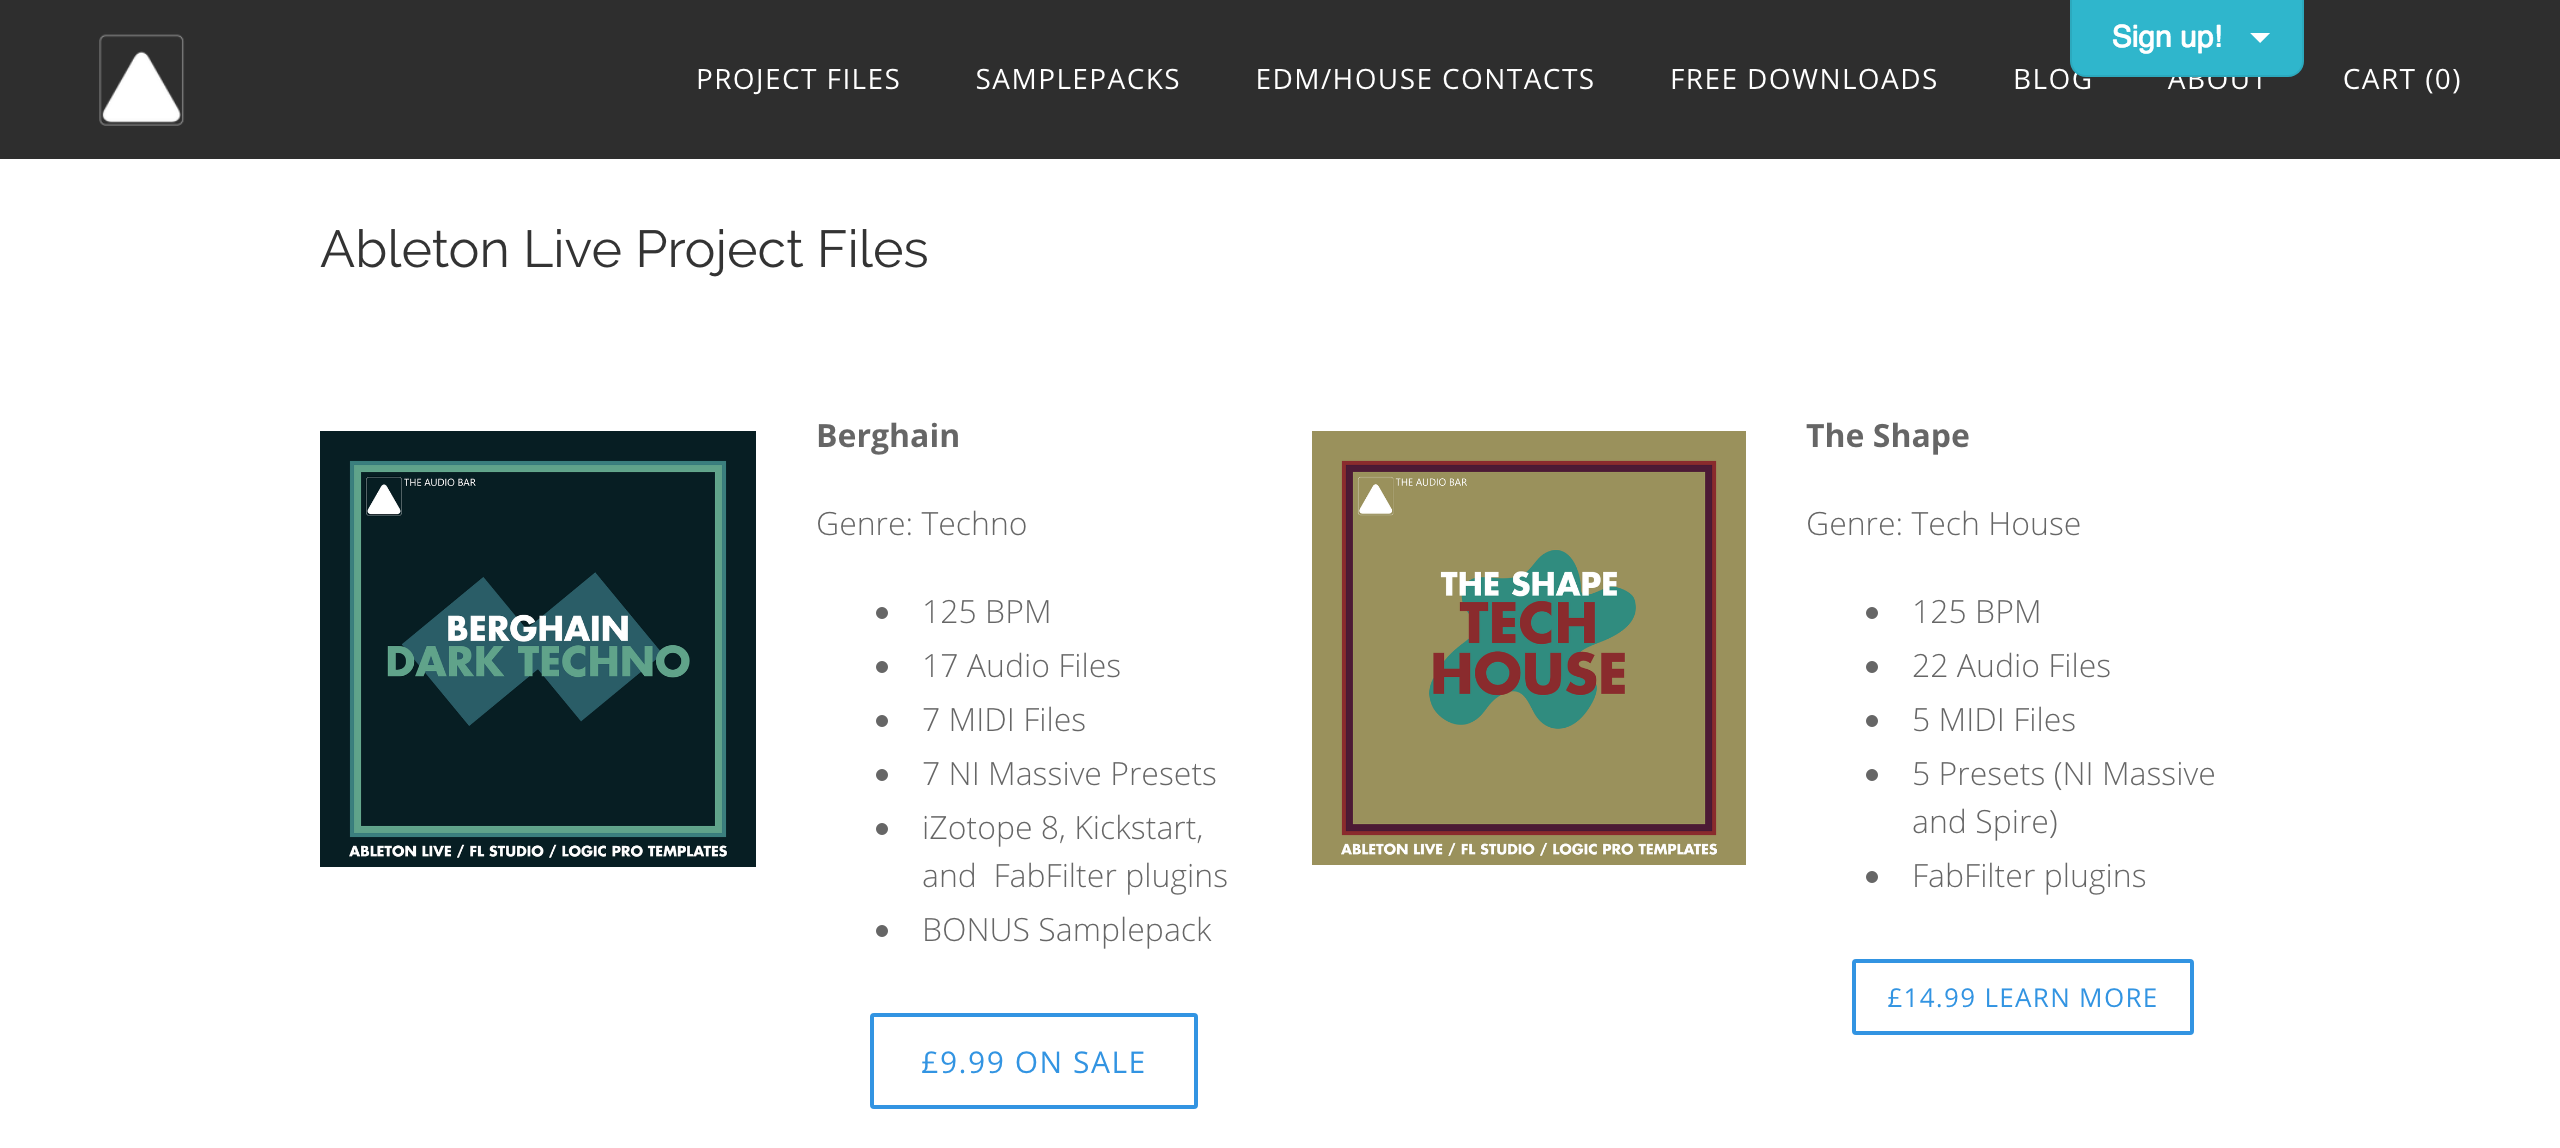
\includegraphics[width=0.9\textwidth]{images/audiobar.png}
    			\label{fig:5}
    		\end{figure}
		\url{https://www.theaudiobar.org/}
	\end{frame}
	%
	\begin{frame}
		\frametitle{Big Bear Audio}
		\framesubtitle{Fundado por Charlie Slee (UK)}
		Invención y manufactura de equipamiento de audio profesional.
		\begin{figure}[h]
    			\centering
    			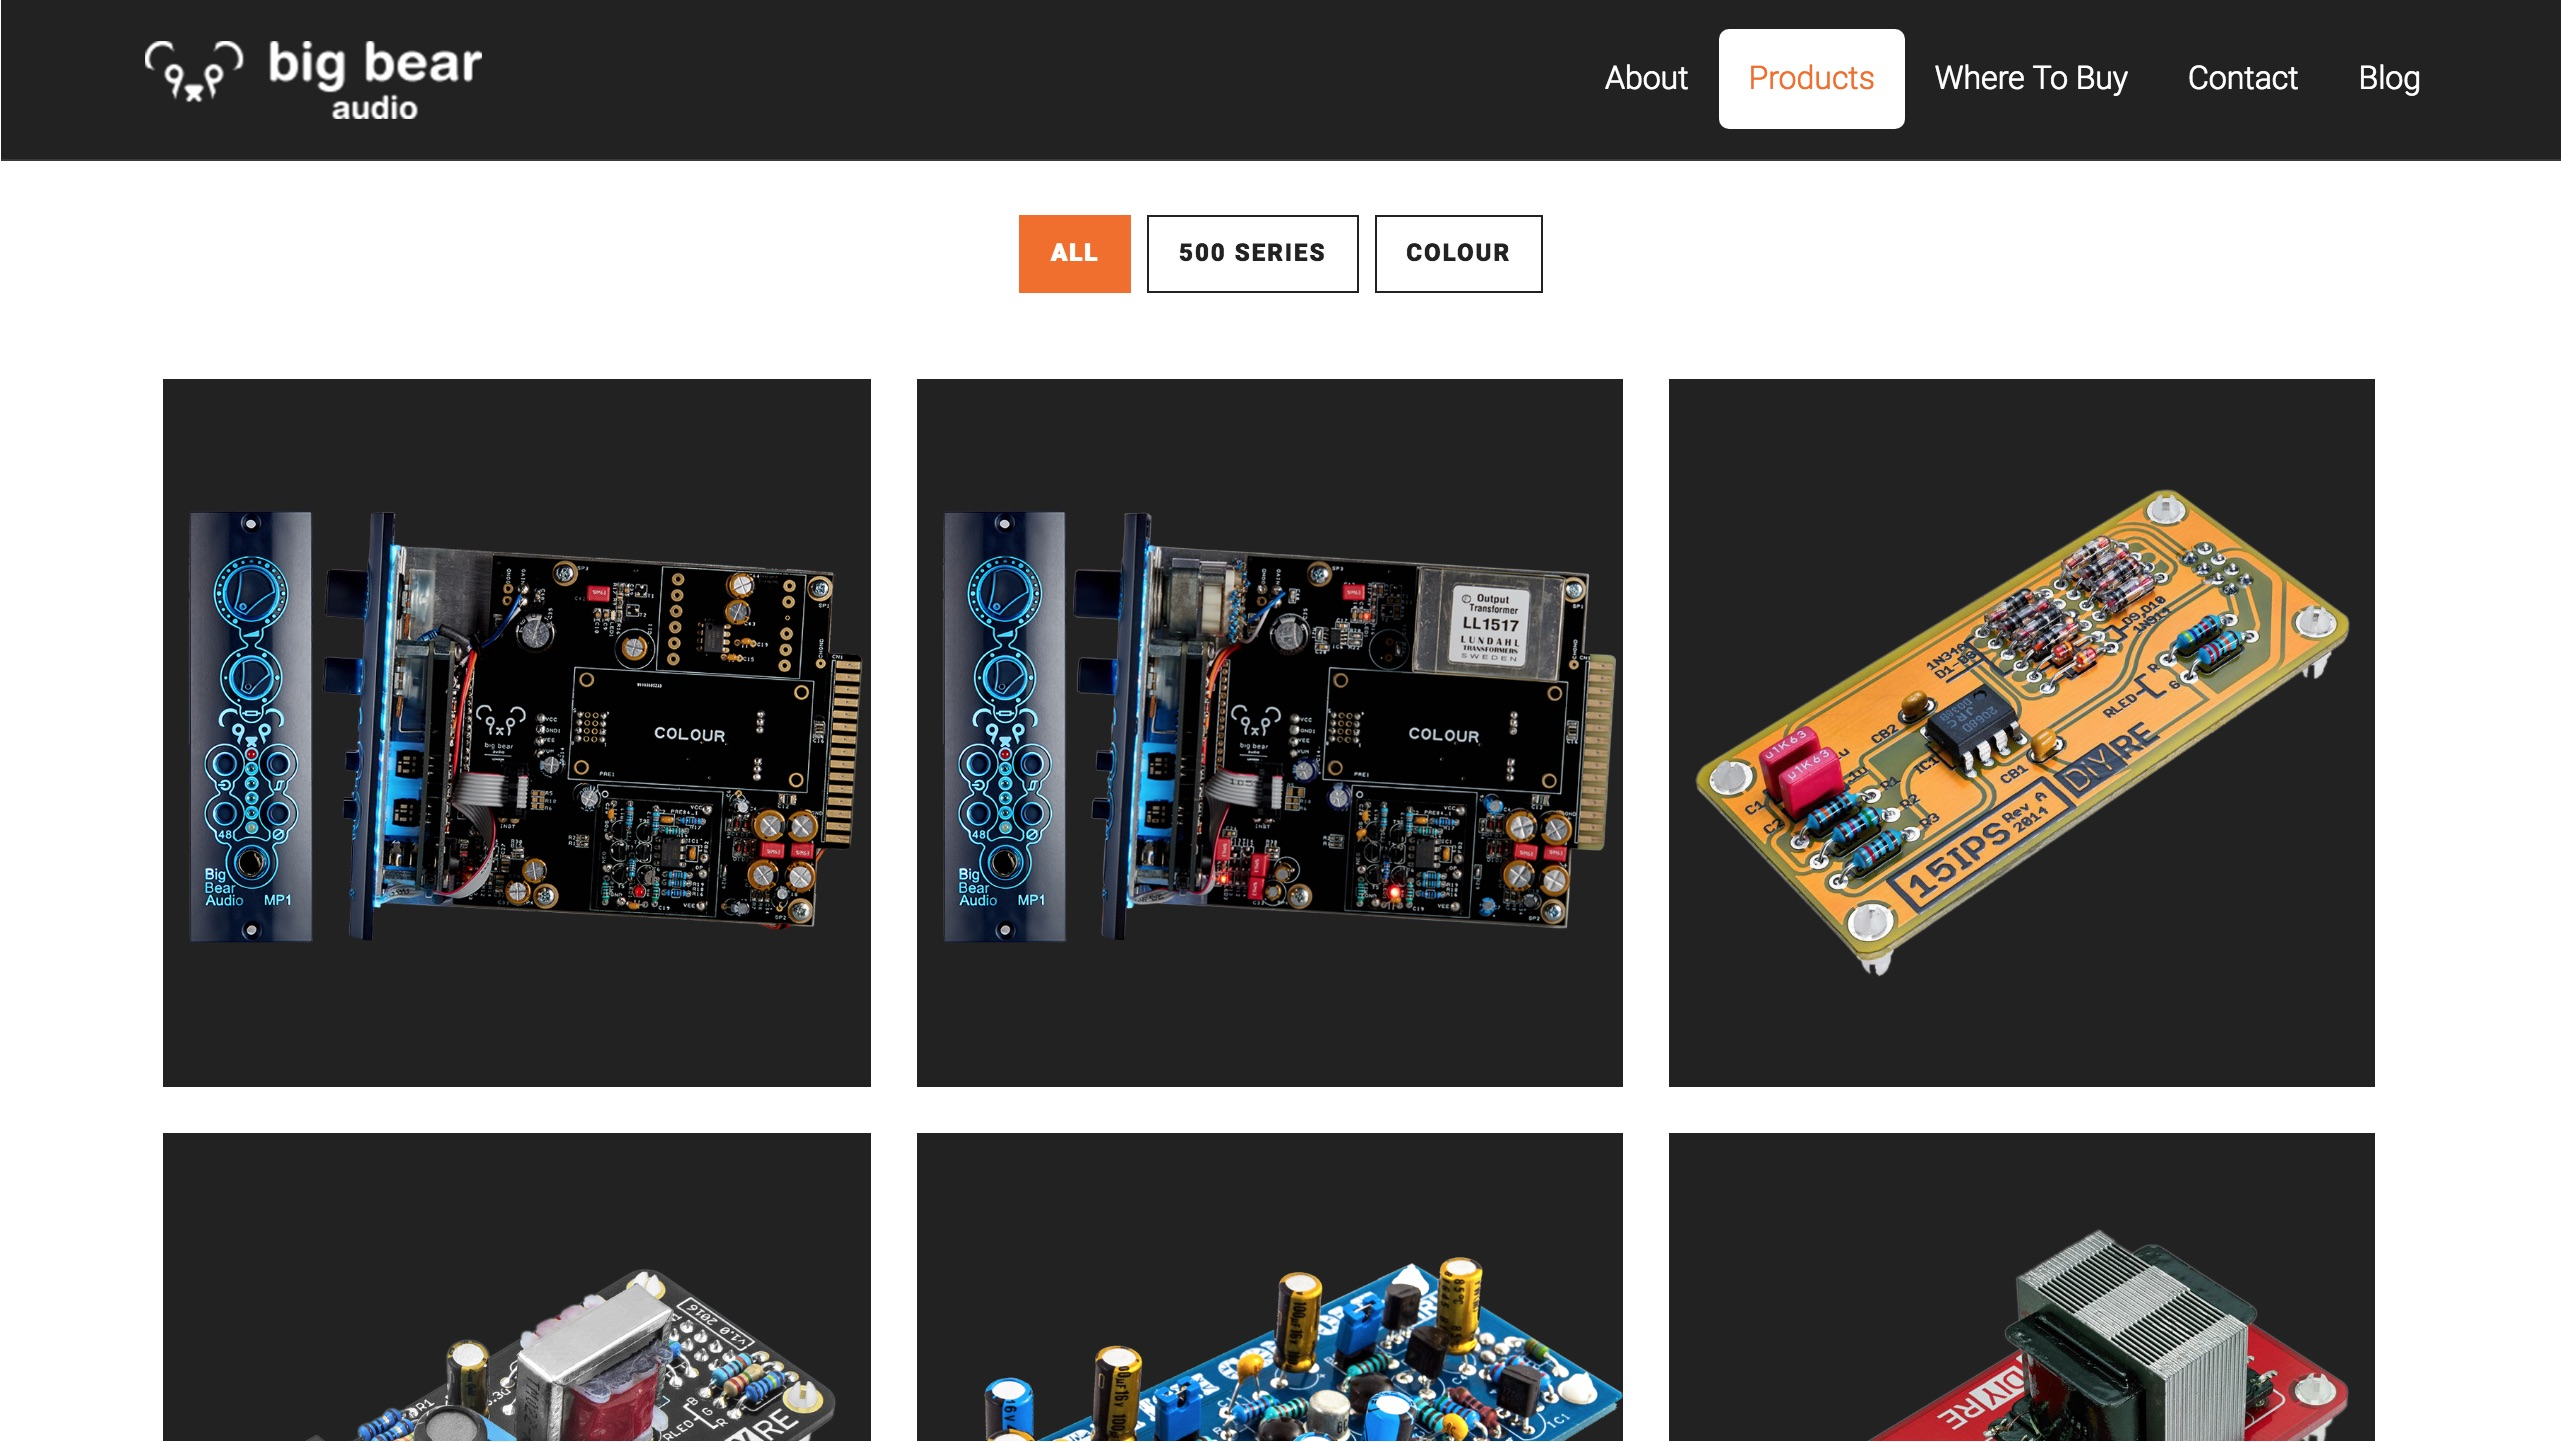
\includegraphics[width=0.7\textwidth]{images/bigbearaudio.jpg}
    			\label{fig:6}
    		\end{figure}
		\url{http://bigbearaudio.com/}
	\end{frame}
	%
	\begin{frame}
		\frametitle{Metafunction}
		\framesubtitle{Fundado por Phelan Kane (UK)}
		Creación de dispositivos Max For Live (M4L), packs, racks y plugins.
		\begin{figure}[h]
    			\centering
    			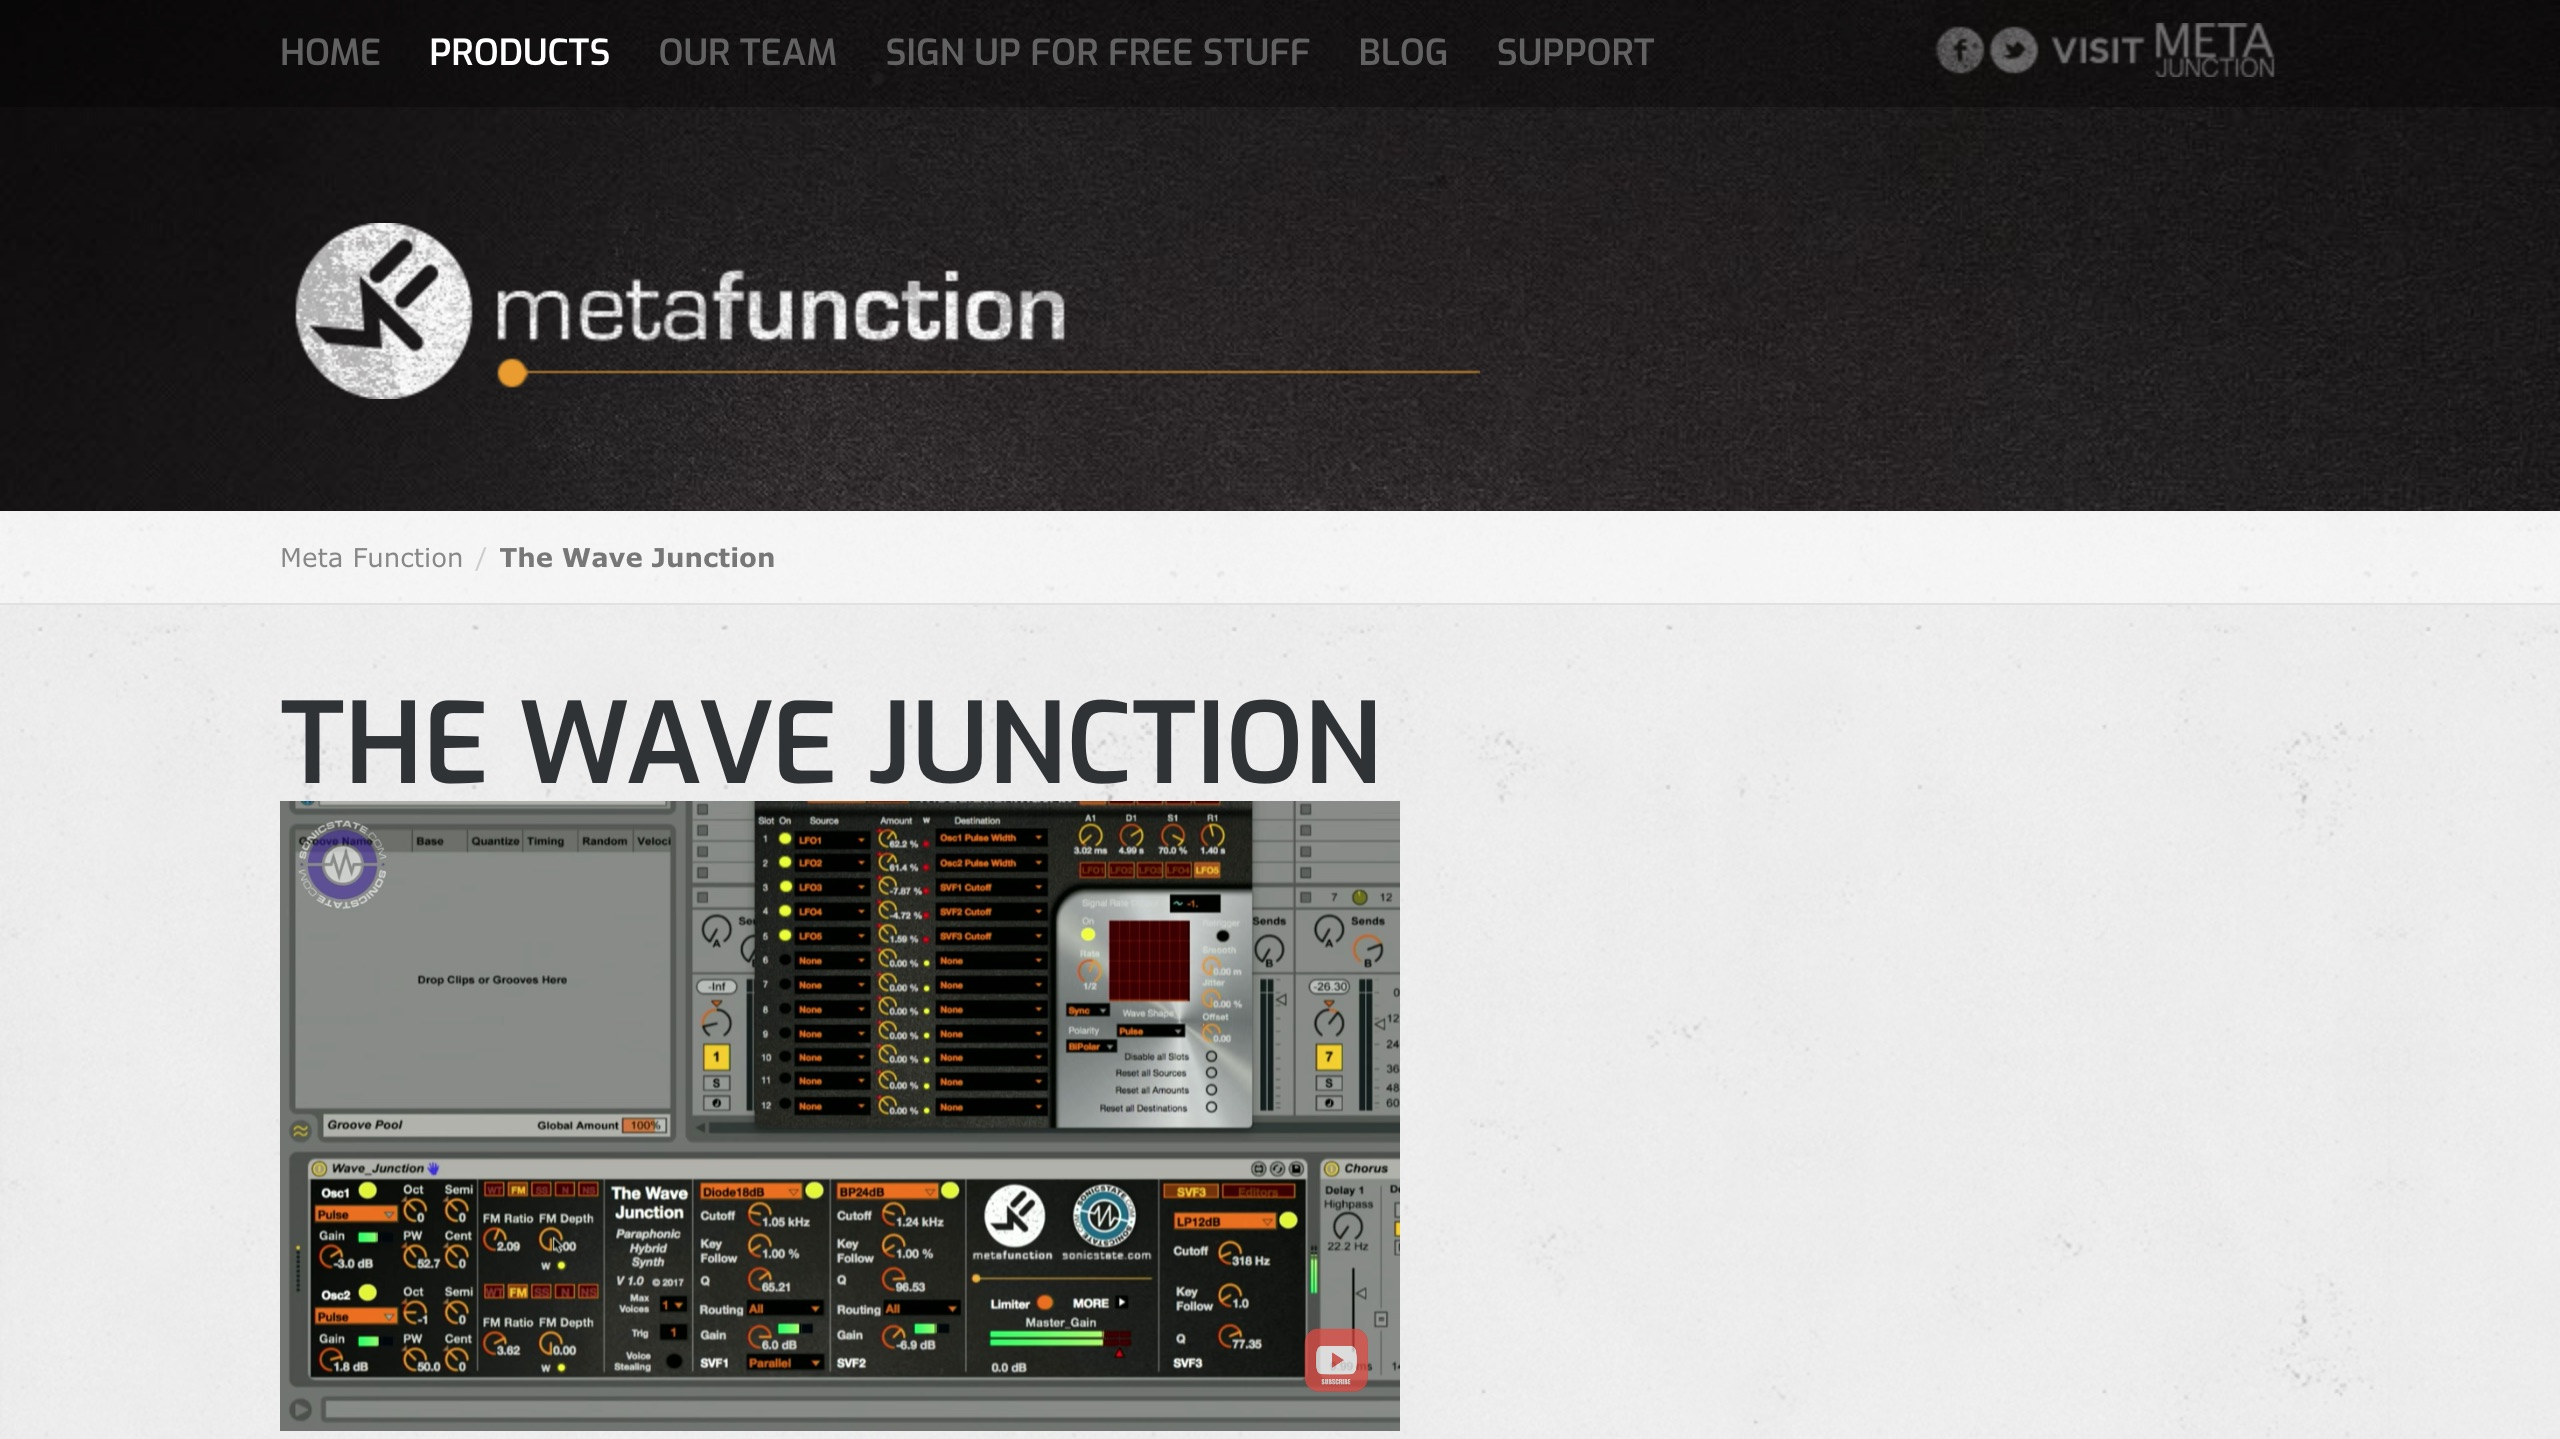
\includegraphics[width=0.7\textwidth]{images/metafunction.jpg}
    			\label{fig:7}
    		\end{figure}
		\url{http://metafunction.co.uk/}
	\end{frame}
	%
	\begin{frame}
		\frametitle{Chirp}
		\framesubtitle{Envío de datos mediante sonido}
		Disponible en Software Developer Kit (SDK).
		\begin{figure}[h]
    			\centering
    			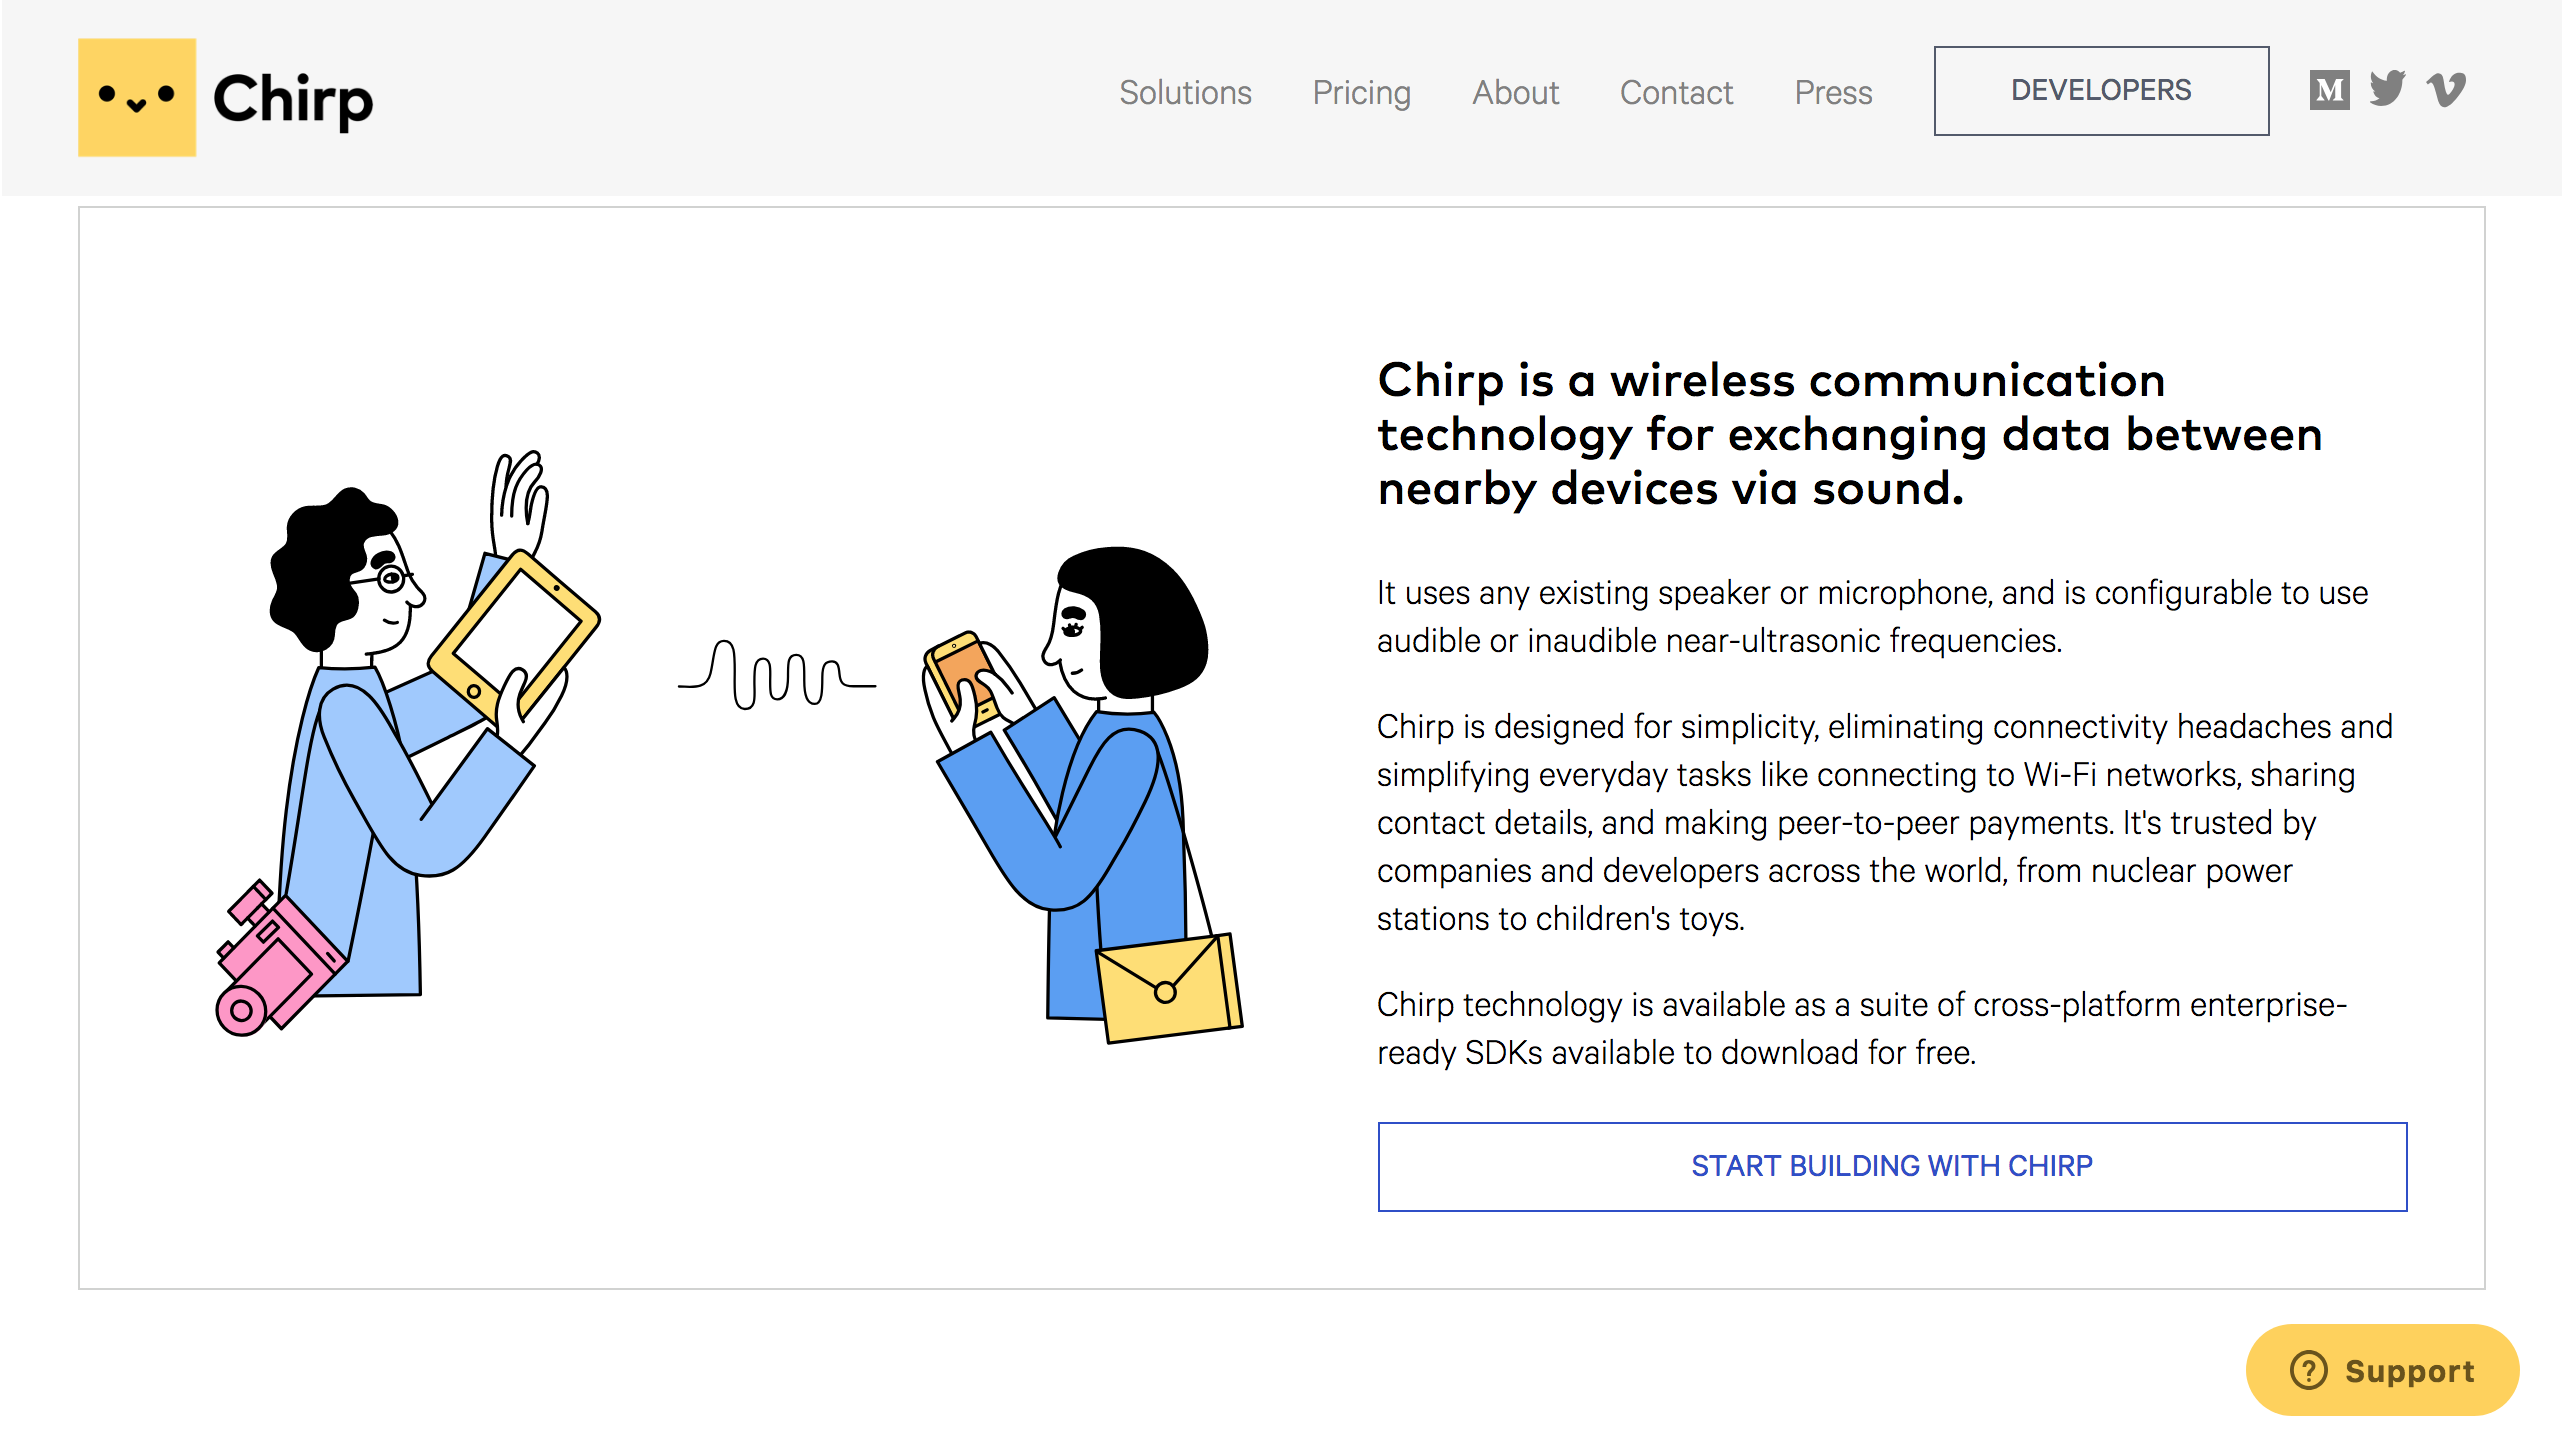
\includegraphics[width=0.7\textwidth]{images/chirp}
    			\label{fig:8}
    		\end{figure}
		\url{https://chirp.io/}
	\end{frame}
	%
	\begin{frame}
		\frametitle{Bela}
		\framesubtitle{Lanzada por el Laboratorio de Instrumentos Aumentados (QMUL)}
		Plataforma para creación de audio responsivo y aplicaciones interactivas
		\begin{figure}[h]
    			\centering
    			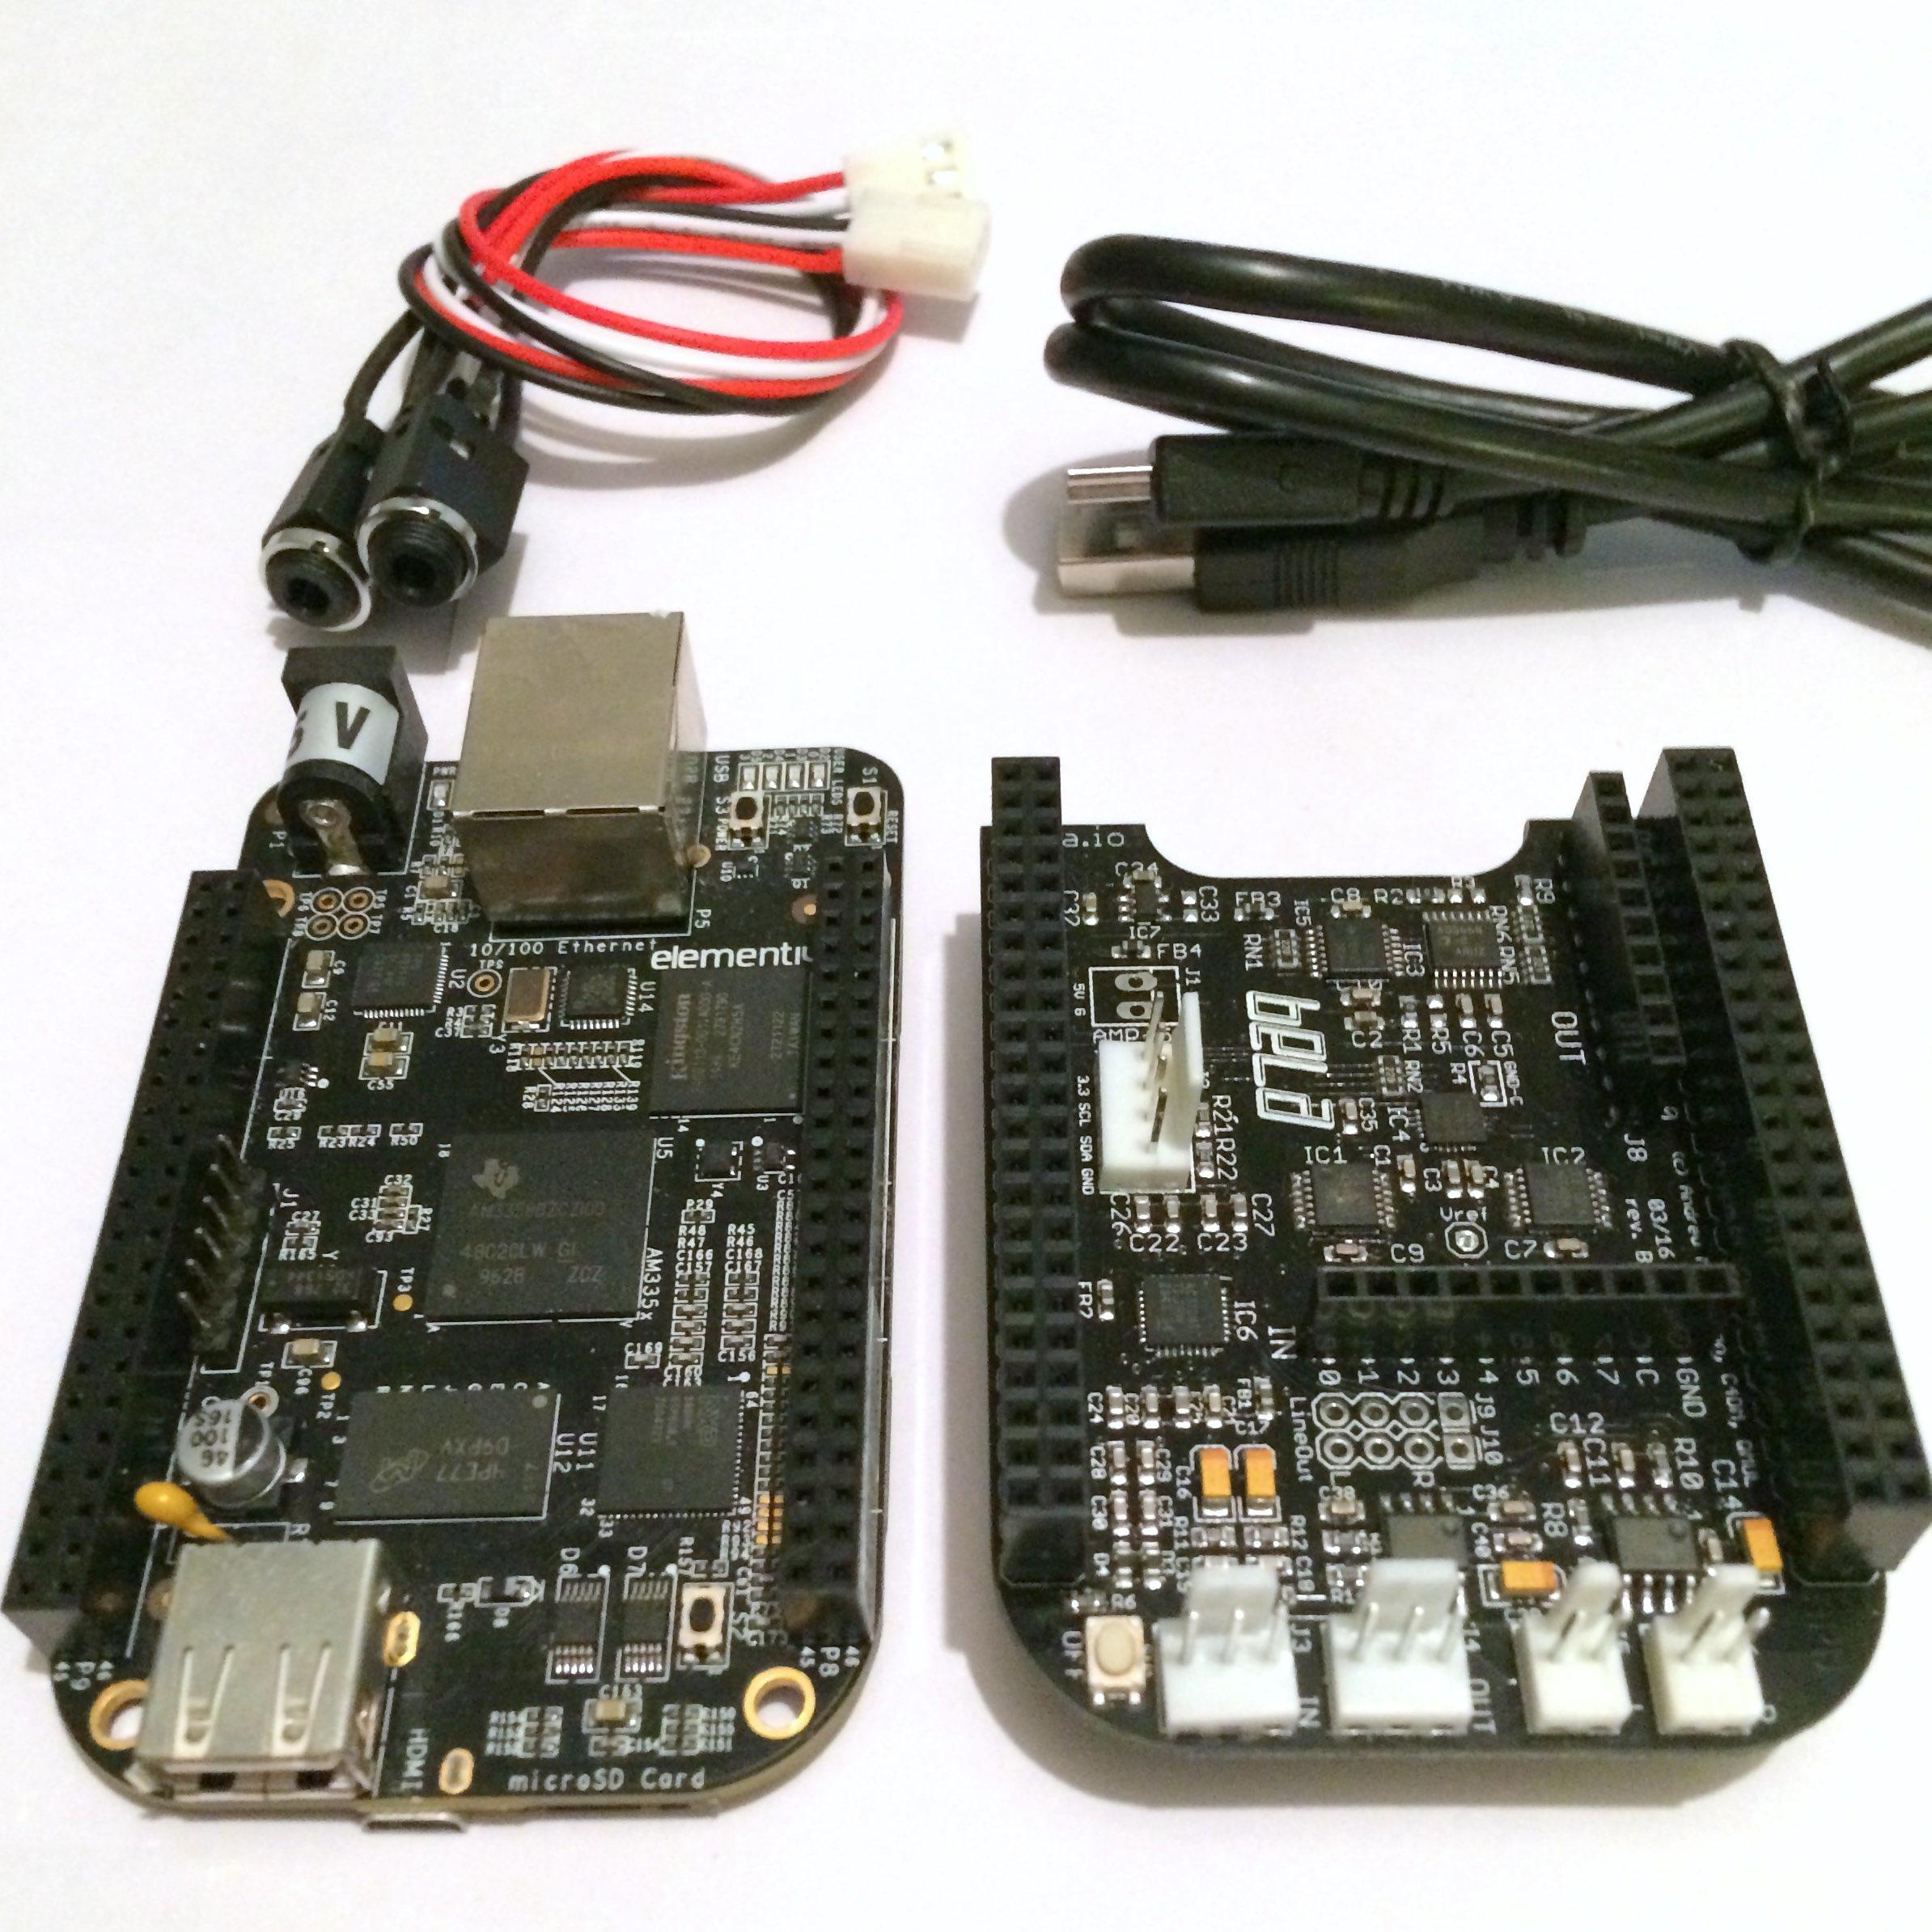
\includegraphics[width=0.4\textwidth]{images/starter-2.jpg}
    			\label{fig:9}
    		\end{figure}
		\url{https://bela.io/}
	\end{frame}
	%
    	\begin{frame}%[allowframebreaks]
        	\frametitle{Bibliografía}
        	{\footnotesize
        		\bibliographystyle{ieeetr}
        		\bibliography{bibliography}
        	}
        \end{frame}
        %
\end{document}